\chapter{ARxCODE}
\label{chap:arxcode} 

\section{Especificaciones}
Python y PyQT
Donde corre y con que performance.
....


\section{Diseño y Desarrollo}
En el IDE EClipse
Funciones enteramente documentadas (Doxigen).
Control de Versiones (GitHub) - graficos de los tiempos de desarrollo. ¿?


\subsection{Arquitectura}
{\bf{Interfaces.}}\\
clases principales: TLE, EphemCODS
\subsection{parametros globales y nomenclatura de la generacion de archivos}
Parametros:\\
\begin{itemize}
 \item satId
 \item fechaIni,fechaFin
 \item TLE/CODS
\end{itemize}

l prototipo de software para el An\'alisis de Riesgo por Colisi\'on con Desechos Espaciales {\it{ARxCODE}}, ser\'a un sistema anexo a las estructuras ya existentes dentro del departamento de Din\'amica Orbital.\\
El mismo se piensa como un intermediario capaz de: detectar los mensajes de alerta CDM provistos por el JSpOC, procesar los datos, generar mejores estimaciones para la posici\'on del desecho, solicitar datos m\'as precisos para la posici\'on de la misi\'on primaria y calcular la PoC. Todo esto a fin de facilitarle a un a un operador analista experto, herramientas para la toma de decisiones o el intercambio de informaci\'on con los organismos externos y el centro de control.\\

\begin{figure}
  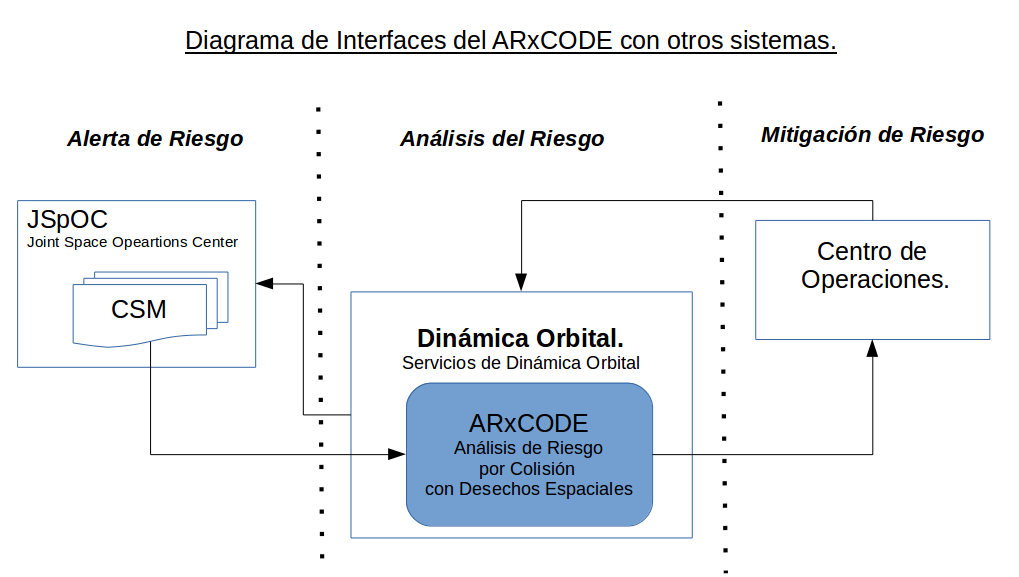
\includegraphics[width=0.8\textwidth]{imagenes/interfasessistemas}
\end{figure}

\subsection*{Requerimientos Funcionales}
\begin{itemize}
\item El sistema deber\'a funcionar en todo momento.\\
\item El software detectar\'a la llegada de un CDM y ser\'a capaz de desglozarlo para extraer la informaci\'on que sea necesaria.\\
\item El software identificar\'a los objetos y solicitar\'a informaci\'on orbital al departamento de Din\'amica Orbital en el caso de la misi\'on principal, y TLEs, en la p\'agina Space-Track, en el caso del desecho.\\
\item El software ajustar\'a la precisi\'on en la posici\'on del desecho y generar\'a la matriz de varianza-covarianza para el mismo.\\
\item El software calcular\'a la PoC.\\
\item El software generar\'a reportes, notificaciones y visualizaciones para facilitar la comprensi\'on y el an\'alisis del riesgo.
\end{itemize}

\subsubsection*{Funcionalidades:}
\begin{itemize}
\item Detectar la recepi\'on de un nuevo mensaje de alerta.\\
\item Extraer la informaci\'on del mensaje y adaptarla al formato necesario.\\
\item Extraer de la web (via spacetrack) los TLEs del desecho involucrado.\\
\item Identificar la misi\'on primaria y solicitar a DO {\color{red}{los datos orbitales precisos necesarios: posici\'on $+$ error}}\\
\item Propagar y ajustar la posici\'on del desecho al TCA, con su error asosciado\\
\item Construir las Matrices Varcorvar.\\
\item Calcular la PoC.\\ 
\end{itemize}


\label{sec:arqydis}
